\subsection{Representations of Variability Models}

\begin{frame}{\insertsubsection} % show list of cfgs, diagrams, text => what are the problems? 
	% this notation is already nice for communication, but semantics matter (for large models, it does not suffice to look sharply)

	% why is this needed? (forward ref?)

	% this section shall teach the relationship between FMs and formulas and FMs and sets (i.e., Damiani 2020, Batory 2005), so: FM semantics

	% also, (valid) total configurations should be explained here (how a computer can check them, this can be checked easily when an FM is encoded eg as runtime variability, but all other SAT-based questions are hard to answer)

	\leftorright{
		\myexample{Natural Language}{
			\tiny ``A \feat{configurable database} has an API that allows for at least one of the request types \feat{Get}, \feat{Put}, or \feat{Delete}.
			Optionally, the database can support \feat{transactions}, provided that the API allows for Put or Delete requests.
			Also, the database targets a supported operating system, which is either \feat{Windows} or \feat{Linux}.''
		}
		\myexample{Configuration Map}{
			\tiny
			\leftandright{
				$\{C,G,W\}$\\
				\hspace{4mm}\vdots\\[1ex]
				$\{C,G,P,D,T,W\}$
			}{
				$\{C,G,L\}$\\
				\hspace{4mm}\vdots\\[1ex]
				$\{C,G,P,D,T,L\}$
			}
		}
		\myexampletight{Feature Model}{
			\centering\tiny
			\featureDiagramConfigurableDatabase
		}
	}{
		\centering
		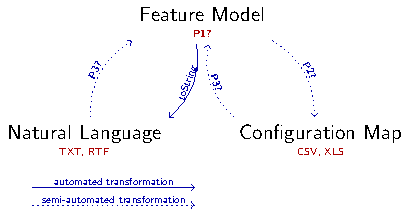
\includegraphics[width=\linewidth]{representations-high-level}

		\mynote{Problems}{
			\begin{enumerate}
				\item[P1] How to express feature models \emph{textually}?
				\item[P2] How to obtain configurations \emph{automatically}?
				\item[P3] \color{gray}{(How to reverse engineer feature models?)}
			\end{enumerate}
		}
	}
\end{frame}

\subsection{Universal Variability Language}

\begin{frame}{\insertsubsection}
	\leftorright{
		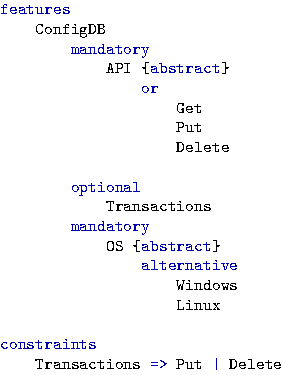
\includegraphics[width=0.7\linewidth]{uvl-model}
	}{
		\centering
		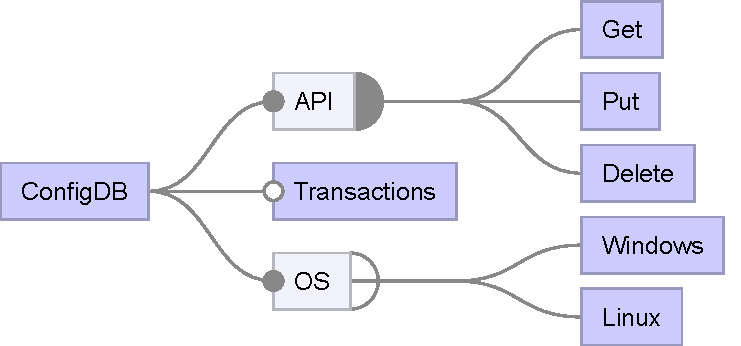
\includegraphics[width=\linewidth]{varied-model}
		$Transactions \pimplies Put \por Delete$
		\mynote{Universal Variability Language (UVL)}{
			\begin{itemize}
				\item textual language for feature modeling
				\item \todots
			\end{itemize}
		}
	}
\end{frame}

\subsection{Recap: Propositional Formulas}

\begin{frame}{\insertsubsection}
	\leftorright{
		\mydefinition{Syntax of Propositional Formulas}{
			A \emph{(propositional) formula} \deutsch{aussagenlogische Formel} is ...
			\begin{itemize}
				\item a \emph{(Boolean) variable} $X$,
    			\item a \emph{negation} $\pnot \phi$ of a formula $\phi$,
    			\item a \emph{conjunction} $(\phi \pand \psi)$ of formulas $\phi$ and $\psi$,
				\item similarly, a \emph{disjunction} $(\phi \por \psi)$, \emph{implication} $(\phi \pimplies \psi)$, or \emph{biimplication} $(\phi \pequals \psi)$.
			\end{itemize}
		}
		\mynote{Operator Precedence: $\pnot$, $\pand$, $\por$, $\pimplies$, $\pequals$}{
			\vspace*{-4ex}
			\begin{align*}
				           &~Transactions \pimplies (Put \por Delete) \\
				\equiv     &~Transactions \pimplies Put \por Delete \\
				\not\equiv &~(Transactions \pimplies Put) \por Delete
			\end{align*}
		}
	}{
		\mydefinition{Informal Semantics of Propositional Formulas}{
			\vspace*{-4ex}
			\begin{equation*}
				\begin{rcases}
					\pnot \phi          \\
					\phi \pand \psi     \\
					\phi \por \psi      \\
					\phi \pimplies \psi \\
					\phi \pequals \psi
				\end{rcases} \text{ means } \begin{cases}
					\text{``not $\phi$''} \\
					\text{``$\phi$ and $\psi$''} \\
					\text{``$\phi$ or $\psi$'' (inclusive)} \\
					\text{``if $\phi$, then $\psi$'' (else?)} \\
					\text{``$\phi$ if and only if $\psi$''}
				\end{cases}
			\end{equation*}
		}
		\mynote{Differences to First-Order Logic}{
			\begin{itemize}
				\item no quantifiers $\forall, \exists$
    			\item no predicates $P(\ldots)$ (e.g., $=$, $>$, $isA$)
    			\item no functions $f(\ldots)$ (e.g., $+$, $\ast$, $typeOf$)
				\item no constants (e.g., $42$, ``hello'')
			\end{itemize}
		}
	}
\end{frame}

\subsection{Propositional Formulas}

\begin{frame}{\insertsubsection}
	\leftandright{
		\only<1-|handout:1>{
			\myexampletight{A Feature Model $FM$ \ldots}{
				\centering\tiny
				\featureDiagramConfigurableDatabase
			}
			\myexample{\ldots as a Propositional Formula $\phi(FM)$}{
				\vspace*{-4ex}
				\small
				\begin{align*}
					\phi(FM) = &~ConfigDB \\
					\pand &~API \pequals ConfigDB \\
					\pand &~Transactions \pimplies ConfigDB \\
					\pand &~OS \pequals ConfigDB \\
					\pand &~Get \por Put \por Delete \pequals API \\
					\pand &~Windows \por Linux \pequals API \\
					\pand &~\pnot (Windows \pand Linux) \\
					\pand &~Transactions \pimplies Put \por Delete
				\end{align*}
			}
		}
	}{
		\only<2-|handout:1>{
			\myexample{Evaluating the Validity of Configurations}{
				\begin{itemize}
					\item $\phi(\{C, G, W\}) = $
						\begin{align*}
							\phi(FM) = &~ConfigDB \\
							\pand &~API \pequals ConfigDB \\
							\pand &~Transactions \pimplies ConfigDB \\
							\pand &~OS \pequals ConfigDB \\
							\pand &~Get \por Put \por Delete \pequals API \\
							\pand &~Windows \por Linux \pequals API \\
							\pand &~\pnot (Windows \pand Linux) \\
							\pand &~Transactions \pimplies Put \por Delete
						\end{align*}
					\item \emph{Invalid} ($\lightning$ no operating system):
						$\{C, G\}$
				\end{itemize}
			}
		}
	}
	%explain intuition behind elements of formula

	%motivate very shortly why this might be nice

\end{frame}

%check valid configuration

\subsection{From Diagram to Formula}

\forestset{
	featureDiagram/.style={
		for tree={
			text depth = 0,
			parent anchor = south,
			child anchor = north,
			draw = drawColor,
			edge = {draw=drawColor},
		}
	}
}

\begin{frame}{-- Algorithm}
	\leftorright{
		$\phi\left(\featureDiagram{Root}\right) = Root$
	
		$\phi\left(\featureDiagram{P[C,optional]}\right) = C \pimplies P$
	
		$\phi\left(\featureDiagram{P[C,mandatory]}\right) = C \pequals P$
	}{
		$\phi\left(\featureDiagram{P[$C_1$,or][\ldots][$C_n$]}\right) = \bigvee_{1 \leq i \leq n} C_i \pequals P$
		
		$\phi\left(\featureDiagram{P[$C_1$,or][\ldots][$C_n$]}\right) = \bigvee_{1 \leq i \leq n} C_i \pequals P \pand \bigwedge_{1 \leq i < j \leq n} \pnot (C_i \pand C_j)$
	}

\end{frame}

\subsection{Conjunctive Normal Form}

\begin{frame}{-- Conjunctive Normal Form}
	CNF is a universal language for saving Boolean formulas, maybe explain it here?
\end{frame}

\begin{frame}{-- Equivalent Transformation}
	
\end{frame}

\begin{frame}{-- DIMACS File Format}
	
\end{frame}

%(state BDD?)
% probably not - (knowledge compilation: there are many nuances between CNF and BDD, maybe discuss?)

\subsection{Other Representations} %variations? these are not only other representations of the same notation

\begin{frame}{\insertsubsection}
	Extended Feature Models
	
	%at the end (what else is there?): in practice, we also have non-Boolean features/attributes/constraints over attributes (more details on efficiency in third block)

	Cardinalities

	Linux/Kconfig % tri-state features

	only requires/excludes constraints
	%there is evidence (Knueppel) that the full expressive power of Boolean formulas is needed for real-world formulas
\end{frame}







% \subsection{Enumerating All Configurations}
% \begin{frame}{\insertsubsection}
% 	\leftandright{
% 		%\myexampletight{}{\centering\includegraphics[width=.75\textwidth]{db-constraint}}
% 		\myexample{26 Valid Configurations}{
% 			\footnotesize
% 			\leftandright{
% 				$\{B,G,W\}$\\
% 				$\{B,P,W\}$\\
% 				$\{B,G,P,W\}$\\
% 				$\{B,D,W\}$\\
% 				$\{B,G,D,W\}$\\
% 				$\{B,P,D,W\}$\\
% 				$\{B,G,P,D,W\}$\\
% 				$\{B,P,T,W\}$\\
% 				$\{B,G,P,T,W\}$\\
% 				$\{B,D,T,W\}$\\
% 				$\{B,G,D,T,W\}$\\
% 				$\{B,P,D,T,W\}$\\
% 				$\{B,G,P,D,T,W\}$
% 			}{
% 				$\{B,G,U\}$\\
% 				$\{B,P,U\}$\\
% 				$\{B,G,P,U\}$\\
% 				$\{B,D,U\}$\\
% 				$\{B,G,D,U\}$\\
% 				$\{B,P,D,U\}$\\
% 				$\{B,G,P,D,U\}$\\
% 				$\{B,P,T,U\}$\\
% 				$\{B,G,P,T,U\}$\\
% 				$\{B,D,T,U\}$\\
% 				$\{B,G,D,T,U\}$\\
% 				$\{B,P,D,T,U\}$\\
% 				$\{B,G,P,D,T,U\}$
% 			}
% 		}
% 	}{}
% \end{frame}

% \subsection{Linux Feature Model}
% \begin{frame}{\insertsubsection}
% 	\vspace{28mm}~\hspace{-15mm}\href{https://dl.acm.org/doi/abs/10.1145/3382025.3414943}{\includegraphics[width=1.2\linewidth,trim=100 510 100 170,clip]{linux-bdd}}
% \end{frame}

% \subsection{Dependencies Modeled in Excel}
% \begin{frame}{\insertsubsection}
% 	\vspace{-7mm}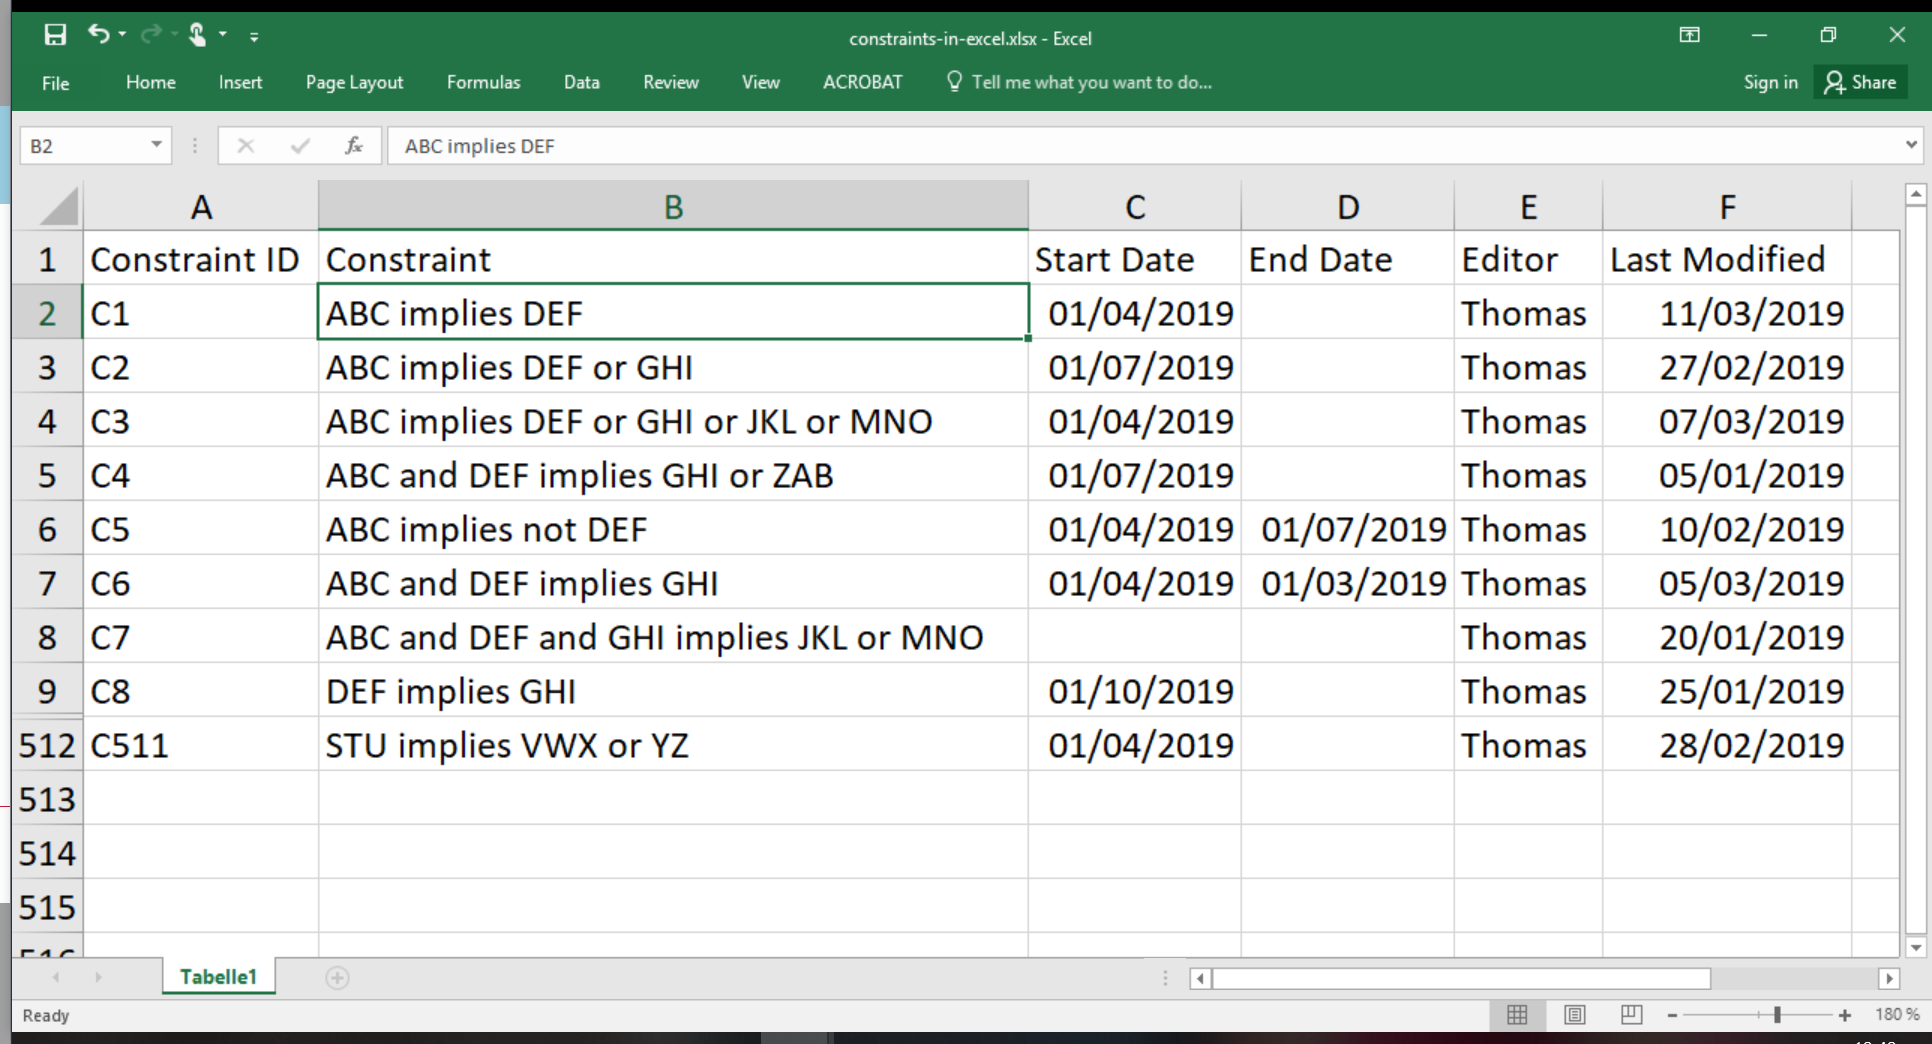
\includegraphics[width=.7\linewidth,trim=10 10 0 10,clip]{constraints-in-excel}
% \end{frame}

\begin{frame}{\insertsubsection}
	\myexampletight{Representations of Variability Models}{
		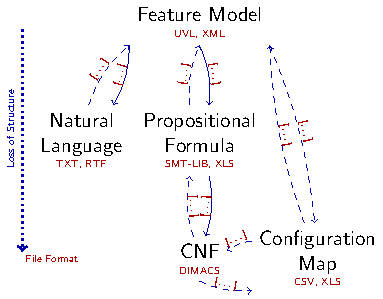
\includegraphics[width=\linewidth]{representations-low-level}

		% describe sat, #sat, allsat
		% describe size of product lines (chico)

		% \myexampletight{Industrial Configuration Spaces \mysource{\evaluatingsharpsatsolvers}}{
		% 	\centering\evaluatingsharpsatsolverslink{\includegraphics[width=\linewidth,page=6,trim=50 210 320 440,clip]{2020/2020-VaMoS-Sundermann}}
		% }

		% feature model of the linux kernel als motivation nutzen, dann recap in testing VL
	}
\end{frame}